\documentclass[11pt]{article}

% ============================================================
%  OTOC / time-evolution proposal for the cross-chip machine
%  Compile on Overleaf (pdfLaTeX). All figures are generated
%  inline with TikZ/pgfplots from MOCK analytic data -- they
%  are placeholders showing what the real plots should look like.
% ============================================================

\usepackage[margin=1in]{geometry}
\usepackage{amsmath, amssymb, bm}
\usepackage{physics}
\usepackage{booktabs}
\usepackage{tikz}
\usepackage{pgfplots}
\pgfplotsset{compat=1.17}
\usetikzlibrary{positioning, decorations.pathmorphing}
\usepackage[colorlinks=true, linkcolor=blue, citecolor=blue]{hyperref}
\usepackage{caption}
\captionsetup{font=small, labelfont=bf}

\newcommand{\eqst}{\varepsilon_{\mathrm{QST}}}
\newcommand{\erzx}{\varepsilon_{\mathrm{RZX}}}
\newcommand{\eloc}{\varepsilon_{\mathrm{2q}}}

\title{Demonstrating coherent cross-chip quantum dynamics:\\
an out-of-time-order-correlator experiment on a modular\\
superconducting processor with QST interconnects}
\author{Draft proposal --- cross\_chips\_sim}
\date{\today}

\begin{document}
\maketitle

\begin{abstract}
We propose a Loschmidt-echo out-of-time-order-correlator (OTOC) experiment on a
modular processor consisting of four (extensible to five or six) 4-qubit chips
connected by microwave cables. The key architectural fact is that the cables
support two operating modes: a direct cross-chip $R_{ZX}$ entangling gate with
depolarizing error $\erzx \approx 0.1$, and full quantum state transfer (QST)
with $\eqst \approx 0.01$. We show that compiling \emph{all} cross-chip
interactions as QST round trips through dedicated port qubits reduces the
effective cross-chip bond error from $0.1$ to $\approx 0.025$, which is the
difference between an operator light cone that fades below the shot-noise
floor mid-module and one that coherently traverses all three cables. The echo protocol reads out a
single qubit, making the modest readout fidelities ($P_1$ success
$0.85$--$0.90$) a trivially correctable scale factor, and its butterfly-free
reference run doubles as a whole-machine benchmark and noise normalizer. We
give the full compilation, qubit layout, error budget, anticipated
(mock) figures, and extensions to 5--6 chips including a periodic ring and a
``butterfly versus cable'' race that directly visualizes the interconnect
beating the emergent Lieb--Robinson velocity of the simulated dynamics.
\end{abstract}

% ============================================================
\section{Goal and headline claim}
% ============================================================

The purpose of this experiment is \emph{not} to measure chemistry observables
(as in the HF/VQE line of work) but to demonstrate that the machine performs
\textbf{coherent many-body time evolution across chip boundaries}. The headline
claim we want a referee to take away:

\begin{quote}
\emph{Quantum information injected on chip~1 spreads ballistically through
Trotterized many-body dynamics, crosses three (or five) optical-quality cable
links, and arrives on the last chip with measurable OTOC signal --- and this is
only possible because cross-chip gates are compiled through state transfer
rather than the native noisy cross-chip entangler.}
\end{quote}

Two figures carry the paper: the light-cone heatmap $C(x,t)$ with the cable
positions marked (Fig.~\ref{fig:lightcone}), and the echo-fidelity comparison
of the two compilation strategies (Fig.~\ref{fig:echofid}).

The document is self-contained: Sec.~\ref{sec:background} defines every
concept from scratch (Heisenberg operators, the OTOC, wave fronts, butterfly
velocity, Lieb--Robinson bounds, scrambling, the Loschmidt echo);
Sec.~\ref{sec:toy} works out an exact two-qubit toy model and a
pen-and-paper argument for how the operator front propagates; the remaining
sections specify the hardware, the compilation, and the experiment we
actually propose to run.

% ============================================================
\section{Background: every object defined}
\label{sec:background}
% ============================================================

All definitions introduced below are collected in the glossary,
Table~\ref{tab:glossary}, for quick reference.

\subsection{Heisenberg picture and operator spreading}

Let $U(t)=e^{-iHt}$ (or a Trotterized circuit approximating it). A local
operator $W$ acting on a single site $b$ evolves in the Heisenberg picture as
\begin{equation}
  W(t) \;=\; U^\dagger(t)\, W\, U(t)
  \;=\; W + it\,[H,W] + \frac{(it)^2}{2!}\,[H,[H,W]] + \cdots
  \label{eq:bch}
\end{equation}
For a Hamiltonian with only nearest-neighbor terms, each nested commutator in
Eq.~\eqref{eq:bch} can extend the \emph{support} of the operator (the set of
sites on which it acts nontrivially) by at most one lattice site. So $W(t)$
starts as a single-site operator and grows into an increasingly nonlocal one
--- this growth of support is called \textbf{operator spreading}, and it is
the microscopic mechanism behind the quantum butterfly effect. Note that
simple expectation values $\expval{W(t)}$ are blind to this growth; one needs
a second operator to \emph{probe} how far $W(t)$ has spread.

\subsection{The OTOC, precisely}
\label{sec:otocdef}

Take two Hermitian \emph{and} unitary local operators (Paulis qualify):
$W$ on site $b$ (the \textbf{butterfly operator}) and $V$ on a distant site
$a$ (the \textbf{probe operator}). At $t=0$ they act on disjoint sites, so
$[W,V]=0$ exactly. The quantity of interest is the \textbf{squared
commutator}
\begin{equation}
  C(t) \;=\; \tfrac{1}{2}\,
  \expval{\,[W(t),V]^\dagger\,[W(t),V]\,}{\psi} \;\geq\; 0 ,
  \label{eq:sqcomm}
\end{equation}
which measures, in the most literal operational sense, how much a
perturbation applied at site $b$ at time $0$ disturbs a measurement at site
$a$ at time $t$. Expanding the commutator and using $W^2=V^2=\mathbb{1}$,
\begin{equation}
  \boxed{\;
  C(t) \;=\; 1 - \mathrm{Re}\, F(t),
  \qquad
  F(t) \;=\; \expval{\,W(t)\,V\,W(t)\,V\,}{\psi} .
  \;}
  \label{eq:otocdef}
\end{equation}
$F(t)$ is the \textbf{out-of-time-order correlator} --- exactly the
``$1 - M(t)\,O\,M(t)\,O$'' structure, with $M(t)=W(t)$ the evolved butterfly
and $O=V$ the probe. The name comes from reading the time arguments of
$W(t)\,V(0)\,W(t)\,V(0)$ left to right: $t \to 0 \to t \to 0$. This ordering
does not appear in any ordinary (causal) response function, and it cannot be
sampled by any single forward-in-time run --- measuring $F(t)$ requires
either an interferometric ancilla or \emph{backward evolution} $U^\dagger$,
which is why our protocol contains an echo.

Interpretation of the two limits:
\begin{itemize}
  \item $F=1$, $C=0$: $W(t)$ still commutes with $V$; the perturbation at
  $b$ has not yet reached $a$. Information is still outside the light cone.
  \item $F\to 0$, $C\to 1$: in a chaotic system at late times $W(t)$ becomes
  an essentially random nonlocal operator, which on average half-commutes and
  half-anticommutes with $V$; the OTOC decays to $\approx 0$ and the squared
  commutator saturates. (Perfect anticommutation would give $F=-1$, $C=2$;
  integrable dynamics can transiently reach such values and revive.)
\end{itemize}

\subsection{Light cone, wave front, and butterfly velocity}
\label{sec:frontdef}

Fix the butterfly site $b$ and scan the probe site $a$; write $x=|a-b|$ for
their separation and regard $C(x,t)$ as a function on the space--time plane.
In every locally interacting system it has the same shape:
\begin{itemize}
  \item an \textbf{outside-the-cone} region ($x \gg v_B t$) where
  $C \approx 0$;
  \item a \textbf{wave front}: the narrow strip around $x \approx v_B t$
  where $C$ rises from $\approx 0$ to its saturation value. The
  \emph{front position} $x_f(t)$ (e.g.\ the contour $C = 0.5\,
  C_{\mathrm{sat}}$) moves ballistically, $x_f \simeq v_B t$, and the
  \emph{front width} $w(t)$ is the distance over which the rise happens;
  \item a \textbf{saturated interior} ($x \ll v_B t$) where the operator has
  fully arrived.
\end{itemize}
The slope of the front defines the \textbf{butterfly velocity} $v_B$: the
speed at which the influence of a local perturbation spreads. Near the front
of a chaotic system the growth is often modeled as exponential,
$C(x,t) \sim \epsilon\, e^{\lambda_L (t - x/v_B)}$, with $\lambda_L$ a
quantum analogue of a Lyapunov exponent (a form strictly derived in
semiclassical/large-$N$ settings; in spin chains the front is sharper and
broadens only sub-ballistically); behind the front it saturates. A
convenient phenomenological form, used for the mock figures below, is
\begin{equation}
  C(x,t) \;\approx\; \tfrac{1}{2}\,C_{\mathrm{sat}}
  \left[\,1 - \tanh\!\Big(\frac{x - v_B t}{w}\Big)\right].
  \label{eq:tanhfront}
\end{equation}
In a brickwork Trotter circuit, time is measured in steps $S$ and $v_B$ in
sites per step; for the kicked Ising model at generic parameters
$v_B \approx 1$ site/step.

\subsection{Lieb--Robinson bound}
\label{sec:lr}

The Lieb--Robinson theorem states that for any Hamiltonian with bounded local
interactions there exist constants $c,\,\xi,\,v_{LR}$ such that
\begin{equation}
  \big\| \,[\,W_b(t),\, V_a\,]\, \big\|
  \;\leq\; c\, \norm{W}\norm{V}\;
  e^{-\left(|a-b| \,-\, v_{LR}\, t\right)/\xi} .
  \label{eq:lr}
\end{equation}
In words: even though the Schr\"odinger equation is not relativistic, locally
interacting quantum matter has an \emph{emergent} speed limit $v_{LR}$;
outside the cone $|a-b| > v_{LR} t$ all commutators --- and hence the OTOC
signal, Eq.~\eqref{eq:sqcomm} --- are exponentially small. The butterfly
velocity always satisfies $v_B \leq v_{LR}$. For circuits the statement is
even sharper and needs no theorem: after $S$ brickwork layers the support of
$W(S)$ has grown by \emph{at most} $S$ sites (a strict, not just exponential,
light cone). Two remarks that matter for this proposal:
\begin{enumerate}
  \item The measured OTOC front (Fig.~\ref{fig:lightcone}) is a direct
  experimental image of an emergent Lieb--Robinson cone.
  \item The bound constrains the \emph{simulated} dynamics only. Hardware
  channels that are not part of the Hamiltonian --- our QST cables --- are
  free to move quantum information faster than $v_{LR}$ of the simulated
  model. That contrast is the point of the ``butterfly--cable race''
  (Sec.~\ref{sec:race}).
\end{enumerate}

\subsection{Scrambling, and why it is not decoherence}

\textbf{Scrambling} is the process by which initially local information
becomes encoded in many-body correlations spread over the entire system: no
local measurement can recover it, but it is still there --- the global
evolution is unitary. The OTOC saturating ($F \to 0$) behind the front is the
standard operational diagnostic of scrambling. Decoherence, by contrast,
leaks information into the environment irreversibly. The echo protocol
distinguishes the two beautifully: backward evolution $U^\dagger$
\emph{refocuses} scrambled information (it is unitary and we control it) but
cannot refocus decohered information. This is precisely why the
butterfly-free echo run measures hardware fidelity, while the ratio of the
two runs isolates the scrambling physics.

\subsection{Loschmidt echo, and the exact identity behind our measurement}
\label{sec:echoderivation}

A \textbf{Loschmidt echo} is any forward-then-backward protocol
$U^\dagger \, P \, U$ with a perturbation $P$ inserted at the turning point.
Our measurement is a single-qubit observable at the end of such an echo, and
it equals the OTOC \emph{exactly} --- no approximation. Derivation: prepare
$\ket{\psi_0}=\ket{0\cdots 0}$, evolve forward, apply the butterfly
$W = X_b$, evolve backward, measure $Z_a$. The final state is
$\ket{\phi} = U^\dagger X_b\, U \ket{\psi_0}$, so the measured expectation is
\begin{equation}
  \expval{Z_a}_{\mathrm{echo}}
  = \bra{\psi_0} \big(U^\dagger X_b U\big)^\dagger Z_a
    \big(U^\dagger X_b U\big) \ket{\psi_0}
  = \bra{\psi_0} W(t)\, Z_a\, W(t) \ket{\psi_0},
\end{equation}
with $W(t) = U^\dagger X_b U$ the Heisenberg butterfly. Now use
$Z_a\ket{\psi_0} = +\ket{\psi_0}$ (the initial state is a $Z_a$ eigenstate)
to append a free $Z_a$ on the right:
\begin{equation}
  \boxed{\;
  \expval{Z_a}_{\mathrm{echo}}
  \;=\; \bra{\psi_0}\, W(t)\, Z_a\, W(t)\, Z_a \,\ket{\psi_0}
  \;=\; F(t)
  \quad\Longrightarrow\quad
  C(t) = 1 - \expval{Z_a}_{\mathrm{echo}} .
  \;}
  \label{eq:echoidentity}
\end{equation}
So the single number we read out \emph{is} the out-of-time-order correlator
$F(t)=\expval{W(t)\,V\,W(t)\,V}$ with $W=X_b$, $V=Z_a$ --- the
``$1-M(t)OM(t)O$'' form --- and the butterfly-free reference run (which would
ideally give $\expval{Z_a}=1$ since $U^\dagger U = \mathbb{1}$) measures the
hardware echo fidelity used for normalization. The identity holds for any
Pauli probe $V$, provided the initial state is prepared as a $+1$ eigenstate
of $V$ (e.g.\ prepare $\ket{+}$ on site $a$ and measure $X_a$ if one wants
$V=X_a$); we use $V=Z_a$ and $\ket{0\cdots0}$ throughout. The identity holds verbatim
for any Pauli probe $V$, provided the initial state is a $+1$ eigenstate of
$V$ (e.g.\ prepare $\ket{+}$ on site $a$ and measure $X_a$); this
generalization is used in the toy-model check below.

\subsection{Trotterization}

We cannot apply $e^{-iHt}$ directly; we approximate it by $S$ discrete steps,
$U(t) \approx (U_{\mathrm{step}})^S$ with $\delta t = t/S$, where
$U_{\mathrm{step}}$ applies the $ZZ$ bond layer and the single-qubit field
layer in sequence. The per-step error is $O(\delta t^2\,\|[H_{ZZ},H_X]\|)$;
for OTOC physics this is benign because a Trotter circuit is itself a
perfectly valid locally interacting dynamics (``kicked Ising'') with its own
front, $v_B$, and scrambling --- we study the circuit as the model, not as an
approximation to be apologized for.

\subsection{Glossary}

\begin{table}[h]
\centering
\small
\begin{tabular}{p{3.4cm} p{10.6cm}}
\toprule
Term & Meaning \\
\midrule
Operator spreading & Growth of the support of a Heisenberg operator $W(t)$, Eq.~\eqref{eq:bch}. \\
Butterfly operator $W$ & The local perturbation ($X_b$ here) whose influence we track. \\
Probe operator $V$ & The distant local observable ($Z_a$ here) used to detect arrival. \\
OTOC $F(t)$ & $\expval{W(t)VW(t)V}$; time order $t\to0\to t\to0$; requires backward evolution. \\
Squared commutator $C(t)$ & $\frac12\expval{|[W(t),V]|^2} = 1-\mathrm{Re}F$; the ``how much does $b$ affect $a$'' number. \\
Light cone & Space--time region $x \lesssim v_B t$ where $C$ is appreciably nonzero. \\
Wave front & The moving strip where $C$ rises from $0$ to saturation; position $x_f\simeq v_B t$, width $w$. \\
Butterfly velocity $v_B$ & Speed of the front; $v_B\approx1$ site/step for kicked Ising. \\
Lieb--Robinson bound & Emergent speed limit $v_{LR}\geq v_B$ for any local dynamics, Eq.~\eqref{eq:lr}. \\
Scrambling & Local info hidden in global correlations; diagnosed by $F\to0$ behind the front. \\
Loschmidt echo & Forward--perturb--backward protocol; its fidelity isolates hardware noise. \\
Trotter step & One $ZZ$-layer $+$ field-layer application; the discrete time unit of the experiment. \\
\bottomrule
\end{tabular}
\caption{Quick-reference glossary for all terms used in this proposal.}
\label{tab:glossary}
\end{table}

% ============================================================
\section{Toy model: the OTOC by hand}
\label{sec:toy}
% ============================================================

\subsection{Two qubits, exactly solvable}

Take $H = J\, Z_1 Z_2$, butterfly $W=X_1$, probe $V=X_2$, state
$\ket{\psi_0}=\ket{00}$. Because $X_1$ anticommutes with $Z_1Z_2$,
\begin{equation}
  W(t) = e^{iHt} X_1 e^{-iHt}
       = X_1\, e^{-2iJt\, Z_1Z_2}
       = \cos(2Jt)\, X_1 \;-\; \sin(2Jt)\, Y_1 Z_2 .
  \label{eq:toyW}
\end{equation}
Read Eq.~\eqref{eq:toyW} as operator spreading in miniature: at $t=0$ the
operator lives on site 1 only; under evolution it rotates weight into
$Y_1Z_2$, a two-site operator. The commutator with the probe is carried
entirely by that grown component:
\begin{equation}
  [\,W(t), X_2\,] = -\sin(2Jt)\,[\,Y_1Z_2,\,X_2\,]
                  = -2i\sin(2Jt)\; Y_1 Y_2 ,
\end{equation}
so the squared commutator and OTOC are
\begin{equation}
  C(t) = \tfrac12 \cdot 4\sin^2(2Jt)\,\expval{(Y_1Y_2)^2} = 2\sin^2(2Jt)
       = 1 - \cos(4Jt),
  \qquad
  \mathrm{Re}\,F(t) = \cos(4Jt).
  \label{eq:toyC}
\end{equation}
Sanity checks: $C(0)=0$ (disjoint operators commute); $C$ first becomes
appreciable on the coupling timescale $1/J$; at $2Jt=\pi/2$ we get $F=-1$,
$C=2$ --- maximal anticommutation, the strongest possible butterfly effect;
and the dynamics is integrable (one bond!), so $C$ revives periodically
instead of saturating. Note the probe choice matters: $V=Z_2$ would give
$C\equiv0$ here, because the grown component $Y_1Z_2$ \emph{commutes} with
$Z_2$ --- for this Hamiltonian all spreading happens in the $X$/$Y$ sector
of site 2. Running the echo protocol of Sec.~\ref{sec:echoderivation} with
the matching probe --- prepare $\ket{0}\!\otimes\!\ket{+}$, evolve, kick
$X_1$, unevolve, measure $X_2$ --- reproduces Eq.~\eqref{eq:toyC} exactly
(verified numerically), and is a recommended first simulation/hardware
check. In the full kicked-Ising experiment the $R_x$ and $R_z$ kicks mix all
Pauli sectors, so the standard choice $V=Z_a$, $\ket{\psi_0}=\ket{0\cdots0}$
detects the front at generic parameters.

\subsection{Why the front moves one site per step}

Now chain the toy: $H_{ZZ} = J\sum_i Z_iZ_{i+1}$ \emph{alone} does not
scramble. Equation~\eqref{eq:toyW} generalizes to
$X_1(t) = \cos X_1 - \sin\, Y_1Z_2$, and there it stops: growing past site 2
would require a nonzero commutator with the next bond $Z_2Z_3$, but both
$X_1$ and $Y_1Z_2$ commute with it (the only piece touching site 2 is
$Z_2$, which commutes with $Z_2Z_3$), so the operator just rotates inside
$\mathrm{span}\{X_1,\, Y_1Z_2\}$ forever and the support never passes
site~2. The transverse kick is what keeps the front moving: a field layer
$e^{-i\theta X_2/2}$ rotates $Z_2 \to \cos\theta\, Z_2 + \sin\theta\, Y_2$,
and the $Y_2$ component \emph{anti}commutes with $Z_2Z_3$, so the next $ZZ$
layer grows the support to site 3. By induction, each (bond layer $+$ kick
layer) step advances the support edge by at most one site --- a two-line
proof of the strict circuit light cone of Sec.~\ref{sec:lr} --- and at
generic angles it advances by essentially exactly one site, giving
$v_B \approx 1$ site/step. The front is not perfectly sharp because the
\emph{weight} carried by the newest edge operators is a product of
$\sin$/$\cos$ factors accumulated along the way; summing the leading paths
gives a front of finite width $w$ that broadens sub-ballistically, which is
what Eq.~\eqref{eq:tanhfront} parameterizes and Fig.~\ref{fig:lightcone}
displays.

\subsection{From toy to proposal}

The proposed experiment is this toy model scaled up: the same $ZZ$ bonds
(three of which happen to cross chip boundaries and are compiled through QST,
Sec.~\ref{sec:compile}), the same kicks, the same echo measurement of
Eq.~\eqref{eq:echoidentity}. Everything measurable reduces to the objects
defined above: the heatmap of $C(a,S)$ shows the light cone, its slope is
$v_B$, its rise is the wave front, its plateau is scrambling, and the
butterfly-free denominator is the Loschmidt-echo fidelity of the machine.

% ============================================================
\section{Hardware model}
% ============================================================

\subsection{Connectivity}

Each chip is a $2\times2$ plaquette; chips are chained by single cables
attached to one ``port-adjacent'' qubit per side
(Fig.~\ref{fig:connectivity}). Cable links (4-chip machine): $(4,5)$, $(7,9)$,
$(11,13)$.

\begin{figure}[h]
\centering
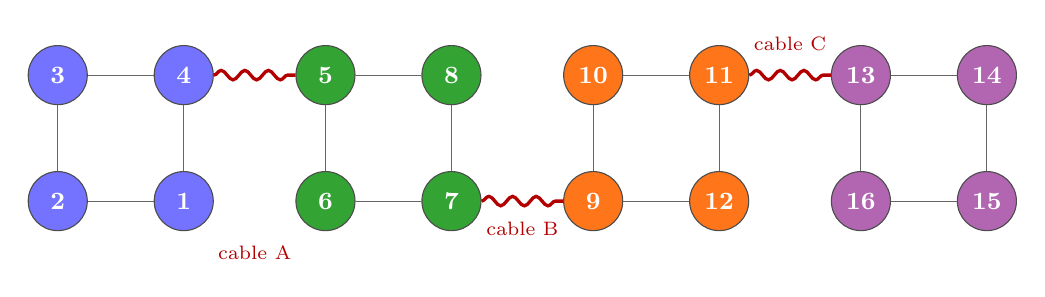
\begin{tikzpicture}[
  q/.style={circle, draw=black!70, minimum size=7.5mm, font=\small\bfseries, inner sep=0pt},
  c1/.style={q, fill=blue!55, text=white},
  c2/.style={q, fill=green!55!black!80, text=white},
  c3/.style={q, fill=orange!80!red!90, text=white},
  c4/.style={q, fill=violet!60, text=white},
  cable/.style={line width=1.2pt, decorate, decoration={snake, amplitude=.6mm, segment length=3mm}, red!70!black},
  wire/.style={black!60}]
  % chip 1
  \node[c1] (q3) at (0,1.6) {3};  \node[c1] (q4) at (1.6,1.6) {4};
  \node[c1] (q2) at (0,0)   {2};  \node[c1] (q1) at (1.6,0)   {1};
  % chip 2
  \node[c2] (q5) at (3.4,1.6) {5}; \node[c2] (q8) at (5.0,1.6) {8};
  \node[c2] (q6) at (3.4,0)   {6}; \node[c2] (q7) at (5.0,0)   {7};
  % chip 3
  \node[c3] (q10) at (6.8,1.6) {10}; \node[c3] (q11) at (8.4,1.6) {11};
  \node[c3] (q9)  at (6.8,0)   {9};  \node[c3] (q12) at (8.4,0)   {12};
  % chip 4
  \node[c4] (q13) at (10.2,1.6) {13}; \node[c4] (q14) at (11.8,1.6) {14};
  \node[c4] (q16) at (10.2,0)   {16}; \node[c4] (q15) at (11.8,0)   {15};
  % intra-chip wires
  \foreach \a/\b in {q3/q4, q2/q1, q3/q2, q4/q1,
                     q5/q8, q6/q7, q5/q6, q8/q7,
                     q10/q11, q9/q12, q10/q9, q11/q12,
                     q13/q14, q16/q15, q13/q16, q14/q15}
    \draw[wire] (\a) -- (\b);
  % cables
  \draw[cable] (q4) -- (q5);
  \draw[cable] (q7) -- (q9);
  \draw[cable] (q11) -- (q13);
  \node[below=1mm of q6, red!70!black, font=\scriptsize] at (2.5,-0.35) {cable A};
  \node[red!70!black, font=\scriptsize] at (5.9,-0.35) {cable B};
  \node[red!70!black, font=\scriptsize] at (9.3,2.0) {cable C};
\end{tikzpicture}
\caption{Four-chip machine. Wavy red edges are cables supporting either a noisy
$R_{ZX}$ ($\erzx\!\approx\!0.1$) or clean QST ($\eqst\!\approx\!0.01$).}
\label{fig:connectivity}
\end{figure}

\subsection{Noise model (numbers taken from the simulation stack)}

\begin{table}[h]
\centering
\begin{tabular}{lll}
\toprule
Channel & Symbol & Value \\
\midrule
Intra-chip 2q depolarizing & $\eloc$ & $0.005$ \\
Intra-chip 1q depolarizing & $\varepsilon_{1q}$ & $10^{-4}$ \\
Cross-chip $R_{ZX}$ depolarizing & $\erzx$ & $0.1$ \\
QST (one transfer over cable) & $\eqst$ & $0.01$ \\
Readout success $P(\text{read }0\,|\,0)$ & $P_0$ & $0.92$--$0.97$ (per qubit) \\
Readout success $P(\text{read }1\,|\,1)$ & $P_1$ & $0.85$--$0.90$ (per qubit) \\
\bottomrule
\end{tabular}
\caption{Error parameters. QST additionally requires the cable mode and the
receiving qubit to start in $\ket{0}$ (single-excitation constraint of the bus).}
\label{tab:noise}
\end{table}

% ============================================================
\section{Compiling cross-chip interactions}
\label{sec:compile}
% ============================================================

\subsection{The QST routing gadget (the workhorse)}

To apply $ZZ(\theta)=e^{-i\theta Z\otimes Z/2}$ between data qubit $a$ (chip
$k$, cable endpoint) and data qubit $b$ (chip $k{+}1$, neighbor of the port
$p$ which is held in $\ket{0}$):
\begin{equation}
  \boxed{\;
  \mathrm{QST}_{a\to p}
  \;\longrightarrow\;
  ZZ(\theta)_{p,b}\ \text{(local)}
  \;\longrightarrow\;
  \mathrm{QST}_{p\to a}
  \;}
\label{eq:gadget}
\end{equation}
The return transfer automatically re-empties $p$, so the gadget is
self-restoring and needs \emph{no} measurement, reset, or feed-forward.
Effective bond error:
\begin{equation}
  \varepsilon_{\mathrm{bond}} \;\approx\; 2\eqst + \eloc \;\approx\; 0.025
  \qquad \text{vs.} \qquad \erzx \approx 0.1 .
\end{equation}
A $4\times$ error reduction per cross-chip bond, which compounds
exponentially with circuit depth.

\subsection{Rejected alternatives (and why)}

\begin{itemize}
  \item \textbf{Direct cross-chip $R_{ZX}$}: $\erzx=0.1$ per bond. With three
  cables and an echo circuit of depth $2S$, the cross-chip error budget alone
  is $0.6S$; the echo falls to the shot-noise floor by $S\approx7$, before
  the light cone can cross the last cable (Sec.~\ref{sec:budget}).
  \item \textbf{Teleported gates via QST/2 Bell pairs}: gate teleportation
  consumes a Bell pair \emph{plus a mid-circuit measurement and feed-forward}.
  With $P_1$ success of $0.85$--$0.90$, each teleported gate inherits a
  $10$--$15\%$ Pauli error from readout --- \emph{worse than the raw
  $R_{ZX}$}. Bell-pair gates become attractive only if readout exceeds
  ${\sim}99\%$.
  \item \textbf{Randomized-measurement OTOCs} (no backward evolution needed):
  require correlating full bitstrings over many qubits, so the ${\sim}10\%$
  per-qubit readout error compounds catastrophically. Not viable here.
\end{itemize}

% ============================================================
\section{The experiment: echo OTOC of a kicked Ising chain}
% ============================================================

\subsection{Model and Trotterization}

We simulate a kicked/transverse-field Ising chain on $N$ data qubits,
\begin{equation}
  H \;=\; J\sum_{\langle i,j\rangle} Z_i Z_j \;+\; h_x \sum_i X_i \;+\; h_z \sum_i Z_i ,
\end{equation}
with one first-order Trotter step
$U_{\mathrm{step}} = \big[\prod_{\langle ij\rangle} ZZ(2J\delta t)\big]
\big[\prod_i R_x(2h_x\delta t) R_z(2h_z\delta t)\big]$.
This is exactly the chained toy model of Sec.~\ref{sec:toy}: the $ZZ$ layer
grows operators across bonds, the kick layer keeps the front moving. The
point $h_z=0$ is integrable (maps to free fermions; sharp ballistic front
with revivals); $h_z\neq0$ breaks integrability (chaotic; front broadens,
OTOC saturates behind it --- genuine scrambling). Cross-chip $ZZ$ bonds use
the gadget of Eq.~\eqref{eq:gadget}; everything else is native intra-chip.

\subsection{Echo (Loschmidt) OTOC protocol}

We run the echo protocol of Sec.~\ref{sec:echoderivation}, which by the exact
identity Eq.~\eqref{eq:echoidentity} measures the OTOC of
Sec.~\ref{sec:otocdef}, $F = \expval{W(t)VW(t)V}$, with butterfly $W=X_b$ and
probe $V=Z_a$:
\begin{enumerate}
  \item Prepare $\ket{\psi_0} = \ket{0\cdots0}$ on the data chain (a $Z_a$
        eigenstate for every $a$, as the identity requires).
  \item Evolve forward: $U = (U_{\mathrm{step}})^S$.
  \item Apply the butterfly $X_b$ on the chip-1 end of the chain
        (or skip it, for the reference run).
  \item Evolve backward: $U^\dagger$ (reversed circuit, negated angles ---
        the QST gadget reverses trivially).
  \item Measure $\expval{Z_a}$ on a \emph{single} qubit $a$; sweep $a$ over the
        chain and $S$ over Trotter depths.
\end{enumerate}
Noiselessly, $\expval{Z_a}_{\text{with }X_b} = F(a,S)$ and
$\expval{Z_a}_{\text{without }X_b} = 1$. With hardware noise, both runs
acquire (to first order in depolarizing noise) the same fidelity prefactor
$f_{\mathrm{echo}}$, so we report the ratio-normalized squared commutator
\begin{equation}
  C(a, S) \;=\; 1 - \frac{\expval{Z_a}_{\text{with }X_b}}
                         {\expval{Z_a}_{\text{without }X_b}}
  \;\approx\; 1 - \frac{f_{\mathrm{echo}}\, F(a,S)}{f_{\mathrm{echo}}}
  \;=\; 1 - F(a,S) ,
\label{eq:normalized}
\end{equation}
i.e.\ precisely the $1 - \expval{W(t)VW(t)V}$ of Eq.~\eqref{eq:otocdef}. The
denominator is simultaneously (i) the whole-circuit Loschmidt-echo fidelity
--- a free whole-machine benchmark --- and (ii) the normalizer that cancels
the depolarizing background, the standard trick that makes OTOCs unusually
noise-robust. Because only one qubit is ever read out, readout error reduces
to a known $2\times2$ confusion matrix (from $P_0, P_1$ of
Table~\ref{tab:noise}) and is inverted exactly.

\subsection{Qubit layout (4-chip machine)}

\begin{table}[h]
\centering
\begin{tabular}{llll}
\toprule
Role & Chip 1 & Chips 2--3 & Chip 4 \\
\midrule
Data chain (11 qubits) & $3\!-\!2\!-\!1\!-\!4$ & $6\!-\!7$ \;and\; $12\!-\!11$ & $16\!-\!15\!-\!14$ \\
Ports (held in $\ket{0}$) & --- & $5$ and $9$ & $13$ \\
Spares & --- & $8$ and $10$ & --- \\
\bottomrule
\end{tabular}
\caption{Chain order: $3,2,1,4 \rightsquigarrow 6,7 \rightsquigarrow 12,11
\rightsquigarrow 16,15,14$. Virtual bonds: $4\!\leftrightarrow\!6$ via port 5;
$7\!\leftrightarrow\!12$ via port 9; $11\!\leftrightarrow\!16$ via port 13.
Butterfly qubit $b=3$ (chain position 1).}
\label{tab:layout}
\end{table}

% ============================================================
\section{Error budget and feasibility}
\label{sec:budget}
% ============================================================

The 11-site open chain of Table~\ref{tab:layout} has 10 bonds: 7 intra-chip
($3\!-\!2$, $2\!-\!1$, $1\!-\!4$; $6\!-\!7$; $12\!-\!11$; $16\!-\!15$,
$15\!-\!14$) and 3 virtual. Each step also applies two field rotations
($R_x$, $R_z$) per qubit. Per Trotter step:
\begin{align}
  \varepsilon_{\mathrm{step}}^{\mathrm{QST}} &\approx
    3 \times 0.025 + 7 \times 0.005 + 2\times11\times 10^{-4} \approx 0.11, \\
  \varepsilon_{\mathrm{step}}^{\mathrm{RZX}} &\approx
    3 \times 0.10 + 7 \times 0.005 + 2\times11\times 10^{-4} \approx 0.34 .
\end{align}
Echo circuits have depth $2S$, so the expected echo fidelity is
$F(S)\approx e^{-2S\,\varepsilon_{\mathrm{step}}}$. With $v_B\approx1$
site/step the front sits near chain position $1+S$ (cables A, B, C lie after
positions 4, 6, 8):

\begin{center}
\begin{tabular}{cccc}
\toprule
$S$ & $F_{\mathrm{QST}}$ & $F_{\mathrm{RZX}}$ & Light-cone reach (butterfly at position 1) \\
\midrule
3  & $0.51$ & $0.13$   & position 4: crossing cable A into chip 2 \\
5  & $0.33$ & $0.034$  & position 6: crossing cable B into chip 3 \\
8  & $0.17$ & $0.0045$ & position 9: crossing cable C into chip 4 \\
10 & $0.11$ & $0.0012$ & position 11: end of chain \\
\bottomrule
\end{tabular}
\end{center}

With $8192$ shots the statistical floor on $\expval{Z}$ is
$\approx 1/\sqrt{8192} \approx 0.011$. The QST compilation stays an order of
magnitude above the floor out to $S=10$; the $R_{ZX}$ compilation reaches the
floor near $S\approx7$ and is already marginal ($3\times$ the floor) by
$S=5$ --- before the butterfly crosses cable C. \textbf{This contrast is the
experiment.}

% ============================================================
\section{Anticipated results (mock figures)}
% ============================================================

All plots below are drawn from analytic mock data --- the tanh front of
Eq.~\eqref{eq:tanhfront} with $v_B \approx 1$ site/step and front width
$w \approx 1.4$ sites --- purely to fix the visual target.

\subsection{Money plot 1: the cross-chip light cone}

\begin{figure}[h]
\centering
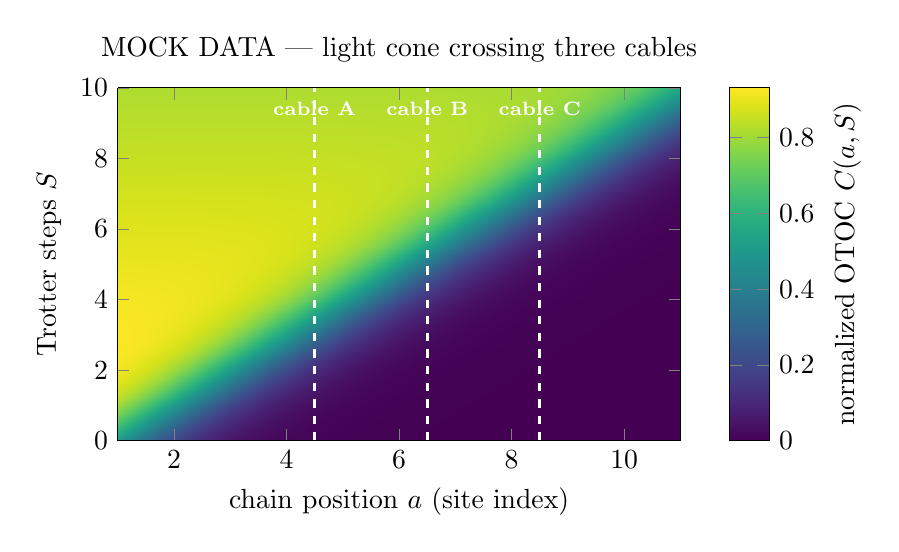
\begin{tikzpicture}
\begin{axis}[
  width=0.72\textwidth, height=0.5\textwidth,
  view={0}{90}, axis on top,
  xlabel={chain position $a$ (site index)}, ylabel={Trotter steps $S$},
  xmin=1, xmax=11, ymin=0, ymax=10,
  colormap/viridis, colorbar,
  colorbar style={ylabel={normalized OTOC $C(a,S)$}},
  title={MOCK DATA --- light cone crossing three cables},
]
% mock light cone: front at x = 1 + v*t, width w, mild decay with depth
\addplot3[surf, shader=interp, domain=1:11, domain y=0:10,
          samples=41, samples y=41]
  { 0.5*(1 - tanh(((x-1) - 1.05*y)/1.4)) * exp(-0.02*y) };
% cable positions (between chain sites 4|5, 6|7, 8|9)
\draw[white, dashed, very thick] (axis cs:4.5,0) -- (axis cs:4.5,10);
\draw[white, dashed, very thick] (axis cs:6.5,0) -- (axis cs:6.5,10);
\draw[white, dashed, very thick] (axis cs:8.5,0) -- (axis cs:8.5,10);
\node[white, font=\scriptsize\bfseries] at (axis cs:4.5,9.4) {cable A};
\node[white, font=\scriptsize\bfseries] at (axis cs:6.5,9.4) {cable B};
\node[white, font=\scriptsize\bfseries] at (axis cs:8.5,9.4) {cable C};
\end{axis}
\end{tikzpicture}
\caption{\textbf{[MOCK]} Normalized OTOC $C(a,S)$, butterfly on site 1
(qubit 3); light cone, wave front, and $v_B$ as defined in
Sec.~\ref{sec:frontdef}. The ballistic front crosses all three cable links
(dashed) without visible degradation --- the direct visual proof of coherent
cross-chip dynamics. The same plot compiled with direct $R_{ZX}$ would fade
to the noise floor around cable~B (Sec.~\ref{sec:budget}).}
\label{fig:lightcone}
\end{figure}

\subsection{Money plot 2: compilation strategy comparison}

\begin{figure}[h]
\centering
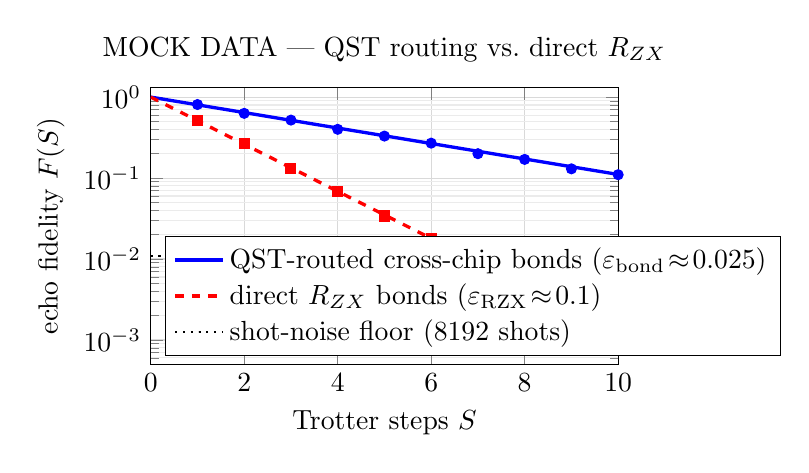
\begin{tikzpicture}
\begin{semilogyaxis}[
  width=0.62\textwidth, height=0.42\textwidth,
  xlabel={Trotter steps $S$}, ylabel={echo fidelity $F(S)$},
  xmin=0, xmax=10, ymin=5e-4, ymax=1.3,
  legend pos=south west, legend cell align=left,
  grid=both, minor grid style={black!8}, major grid style={black!15},
  title={MOCK DATA --- QST routing vs.\ direct $R_{ZX}$},
]
% theory curves: F = exp(-2 S eps_step) with eps = 0.11 (QST) / 0.34 (RZX)
\addplot[blue, very thick, domain=0:10, samples=60] {exp(-0.22*x)};
\addlegendentry{QST-routed cross-chip bonds ($\varepsilon_{\mathrm{bond}}\!\approx\!0.025$)}
\addplot[red, very thick, dashed, domain=0:10, samples=60] {exp(-0.67*x)};
\addlegendentry{direct $R_{ZX}$ bonds ($\erzx\!\approx\!0.1$)}
\addplot[black, dotted, thick, domain=0:10] {0.011};
\addlegendentry{shot-noise floor ($8192$ shots)}
% markers: fake experimental points with small scatter around the curves
\addplot[blue, only marks, mark=*, mark size=1.8pt] coordinates
  {(1,0.81) (2,0.63) (3,0.52) (4,0.40) (5,0.33) (6,0.27) (7,0.20) (8,0.17) (9,0.13) (10,0.11)};
\addplot[red, only marks, mark=square*, mark size=1.8pt] coordinates
  {(1,0.51) (2,0.27) (3,0.13) (4,0.068) (5,0.034) (6,0.018) (7,0.009)};
\end{semilogyaxis}
\end{tikzpicture}
\caption{\textbf{[MOCK]} Butterfly-free echo fidelity vs.\ depth for the two
compilations of the \emph{same} physical circuit. The gap is the
quantitative ``power of the interconnect'' statement.}
\label{fig:echofid}
\end{figure}

\subsection{Supporting plot: chaotic vs.\ integrable spreading}

\begin{figure}[h]
\centering
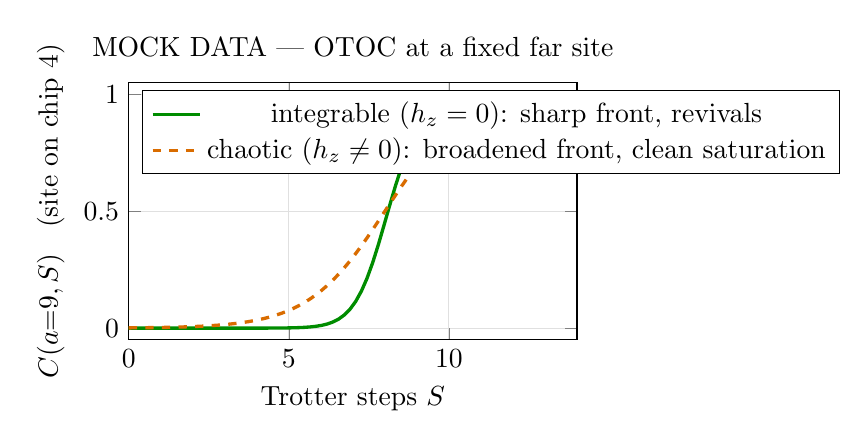
\begin{tikzpicture}
\begin{axis}[
  width=0.6\textwidth, height=0.4\textwidth,
  xlabel={Trotter steps $S$}, ylabel={$C(a{=}9,S)$ \; (site on chip 4)},
  xmin=0, xmax=14, ymin=-0.05, ymax=1.05,
  legend pos=north west, grid=major, major grid style={black!12},
  title={MOCK DATA --- OTOC at a fixed far site},
]
\addplot[green!55!black, very thick, domain=0:14, samples=80]
  {0.5*(1+tanh((x-8)/0.9)) * (0.95 + 0.05*cos(deg(1.9*x)))};
\addlegendentry{integrable ($h_z=0$): sharp front, revivals}
\addplot[orange!85!black, very thick, dashed, domain=0:14, samples=80]
  {0.5*(1+tanh((x-8)/2.4))};
\addlegendentry{chaotic ($h_z\neq0$): broadened front, clean saturation}
\end{axis}
\end{tikzpicture}
\caption{\textbf{[MOCK]} Fixing the measurement qubit on chip 4 and sweeping
depth distinguishes integrable and chaotic dynamics --- physics content beyond
a hardware benchmark.}
\label{fig:chaos}
\end{figure}

% ============================================================
\section{Expanding to 5--6 chips: the fun part}
% ============================================================

With 5--6 chips the chain extends to ${\sim}13$--$15$ data qubits
(interior chips contribute 2 data + 1 port + 1 spare each), and several
qualitatively new experiments open up.

\subsection{Longer light cone and scrambling saturation}
Five cables instead of three. The error budget scales gently: each extra
interior chip adds two data sites, i.e.\ one virtual bond ($+0.025$/step),
one local bond ($+0.005$/step), and two qubits of field-layer noise. At 6
chips (15-site chain: 9 intra-chip $+$ 5 virtual bonds)
$\varepsilon_{\mathrm{step}} \approx 5\times0.025 + 9\times0.005 +
2\times15\times10^{-4} \approx 0.17$, so the echo at $S=10$ is
$e^{-3.5}\approx 3\%$ --- marginal but ${\sim}5\times$ above the floor with
$3\times10^4$ shots ($1/\sqrt{3\times10^4}\approx0.006$). The payoff: enough
depth \emph{and} length to see the OTOC front pass \emph{and} saturate
behind it, i.e.\ genuine scrambling, not just transport.

\subsection{Ring closure: periodic boundary conditions}
If chip 6 can be cabled back to chip 1, the machine realizes a
\emph{periodic} chain --- something planar fixed layouts cannot do without
massive swap overhead. Signatures: the two counter-propagating OTOC fronts
launched by one butterfly \emph{collide on the far side of the ring}, giving
a distinctive interference bump at the antipodal site at
$t \approx L/(2v_B)$; momentum quantization becomes visible in quench
spectroscopy. This is a demo only a modular machine does cheaply.

\subsection{The butterfly--cable race (recommended headline demo)}
\label{sec:race}
Run two protocols simultaneously on one machine:
\begin{itemize}
  \item \textbf{Lane 1 (dynamics):} the butterfly spreads through Trotter
  evolution at the emergent Lieb--Robinson velocity $v_B \approx 1$
  site/step.
  \item \textbf{Lane 2 (interconnect):} a reference excitation is relayed down
  the \emph{spare/port qubits} by bare QST hops, at one \emph{chip} per hop.
\end{itemize}

\begin{figure}[h]
\centering
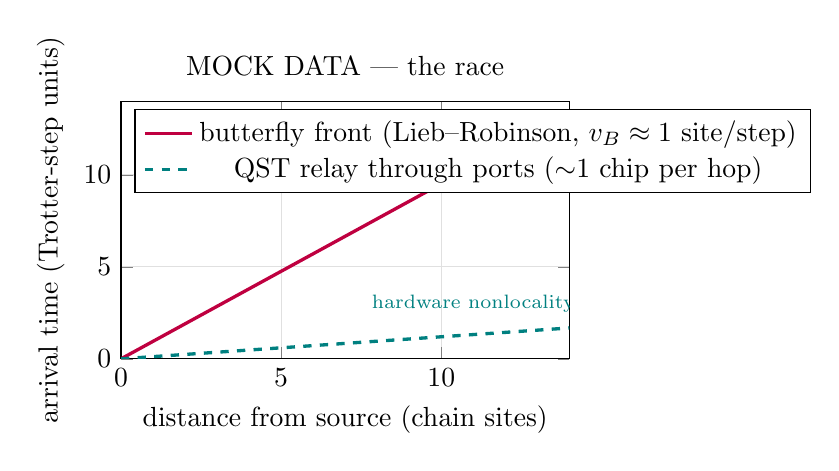
\begin{tikzpicture}
\begin{axis}[
  width=0.6\textwidth, height=0.4\textwidth,
  xlabel={distance from source (chain sites)},
  ylabel={arrival time (Trotter-step units)},
  xmin=0, xmax=14, ymin=0, ymax=14,
  legend pos=north west, grid=major, major grid style={black!12},
  title={MOCK DATA --- the race},
]
\addplot[purple, very thick, domain=0:14] {x/1.05};
\addlegendentry{butterfly front (Lieb--Robinson, $v_B \approx 1$ site/step)}
\addplot[teal, very thick, dashed, domain=0:14] {0.12*x};
\addlegendentry{QST relay through ports ($\sim$1 chip per hop)}
\node[font=\scriptsize, purple] at (axis cs:9.5,12.3) {simulated locality};
\node[font=\scriptsize, teal] at (axis cs:11,3.0) {hardware nonlocality};
\end{axis}
\end{tikzpicture}
\caption{\textbf{[MOCK]} Arrival time vs.\ distance for the two lanes. The
interconnect beats the light cone of the simulated Hamiltonian by an order of
magnitude --- a one-plot statement that modular hardware adds a resource
(long-range quantum channels) that the simulated physics does not have.}
\label{fig:race}
\end{figure}

\subsection{Colliding butterflies}
With $\geq 5$ chips there is room to launch butterflies from \emph{both} ends
and watch the two OTOC fronts collide mid-machine (on a middle chip). The
collision region shows enhanced operator weight and, at the integrable point,
transmission of fronts through each other --- a clean, visual many-body
scattering experiment.

% ============================================================
\section{Error mitigation stack}
% ============================================================

\begin{enumerate}
  \item \textbf{Readout}: exact $2\times2$ confusion-matrix inversion on the
  single measured qubit, calibrated from $P_0, P_1$.
  \item \textbf{Normalization}: Eq.~\eqref{eq:normalized} cancels the
  depolarizing background to first order.
  \item \textbf{ZNE on the cables}: inserting identity QST round-trip pairs
  ($a \to p \to a$) scales cross-chip noise in clean units of $2\eqst$ --- an
  unusually well-controlled noise-amplification knob unique to this
  architecture.
  \item \textbf{CDR}: the existing Clifford-data-regression machinery
  (\texttt{main\_cursor\_lib}) applies directly since the Trotter circuits are
  Clifford at $J\delta t, h\delta t \in \{0, \pi/4\}$.
\end{enumerate}

% ============================================================
\section{Milestones}
% ============================================================

\begin{enumerate}
  \item \textbf{M1 --- gadget validation}: single virtual bond (chips 1--2);
  process fidelity of Eq.~\eqref{eq:gadget} vs.\ direct $R_{ZX}$.
  \item \textbf{M2 --- domain-wall quench}: prepare
  $\ket{0\cdots0\,1\cdots1}$, forward evolution only, measure
  $\expval{Z_i(t)}$ profile crossing the cables. Half the depth of the echo;
  validates layout, calibration, and mitigation.
  \item \textbf{M3 --- echo OTOC, 4 chips}: Figs.~\ref{fig:lightcone}
  and~\ref{fig:echofid}; then the integrable-vs-chaotic sweep of
  Fig.~\ref{fig:chaos}.
  \item \textbf{M4 --- 5/6 chips}: extended light cone; ring and/or
  butterfly--cable race (Fig.~\ref{fig:race}); colliding butterflies.
\end{enumerate}

\end{document}